\begin{figure}
  \centering
  \begin{tabular}{cc}
    % top row
    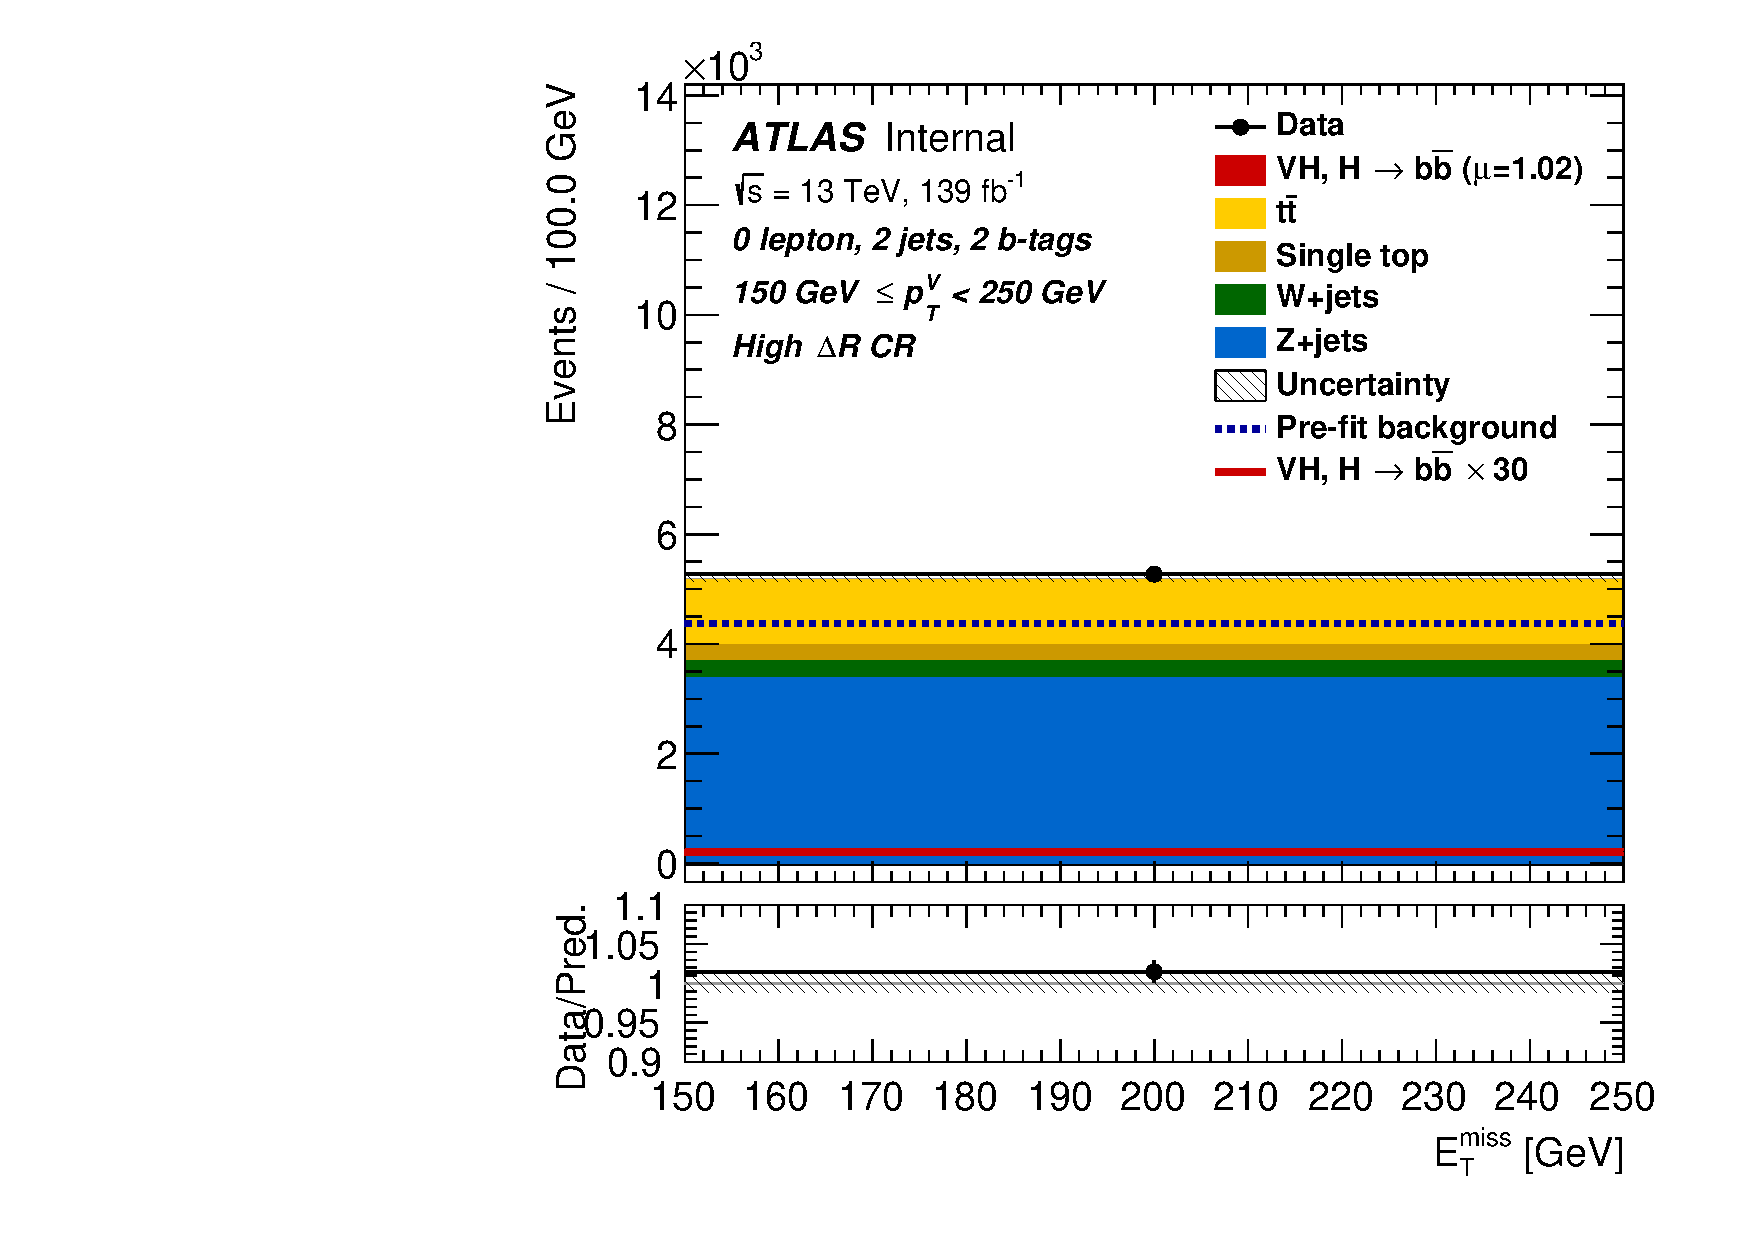
\includegraphics[width=.49\textwidth]{final_fit_mva/postfit/Region_BMax250_BMin150_Y6051_DCRHigh_T2_L0_distMET_J2_GlobalFit_unconditionnal_mu1}%
    & 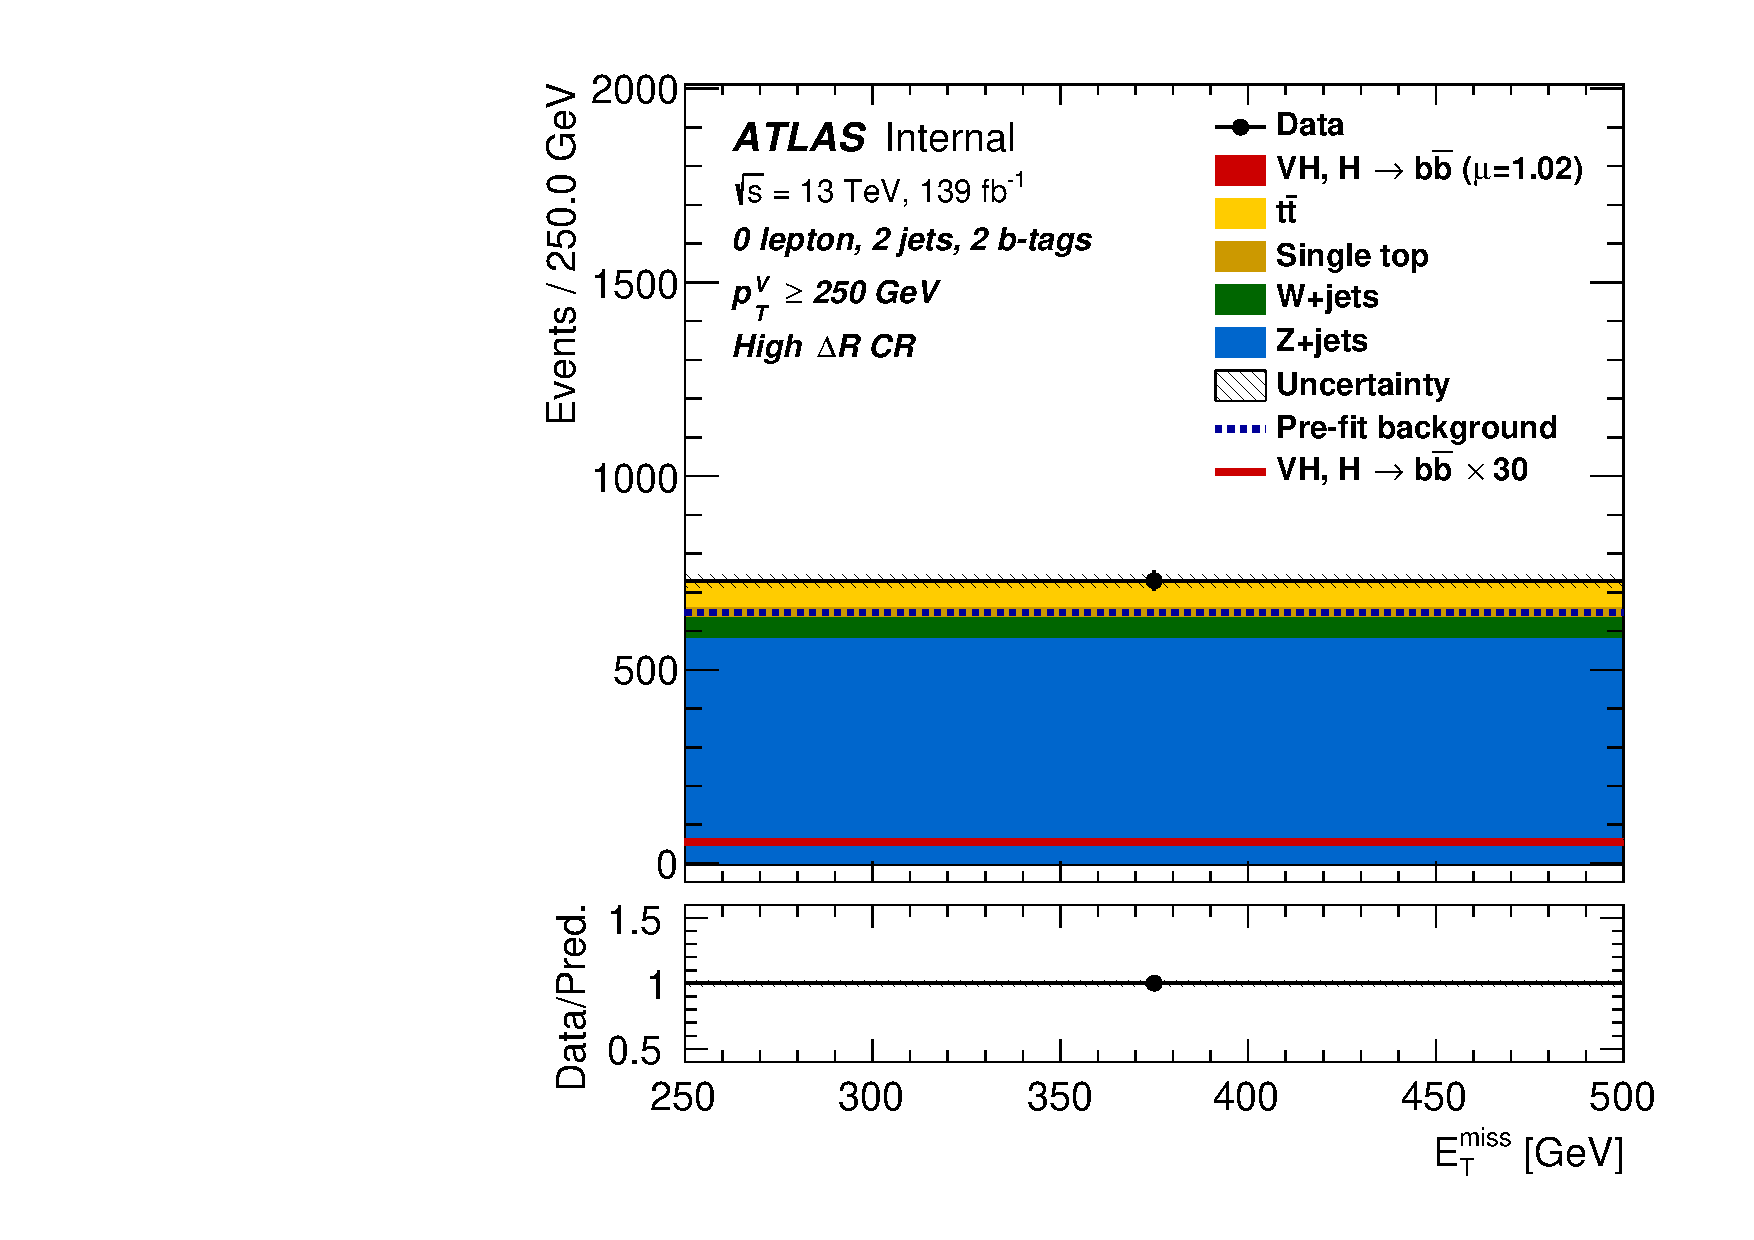
\includegraphics[width=.49\textwidth]{final_fit_mva/postfit/Region_BMin250_Y6051_DCRHigh_T2_L0_distMET_J2_GlobalFit_unconditionnal_mu1} \\

    % middle row
    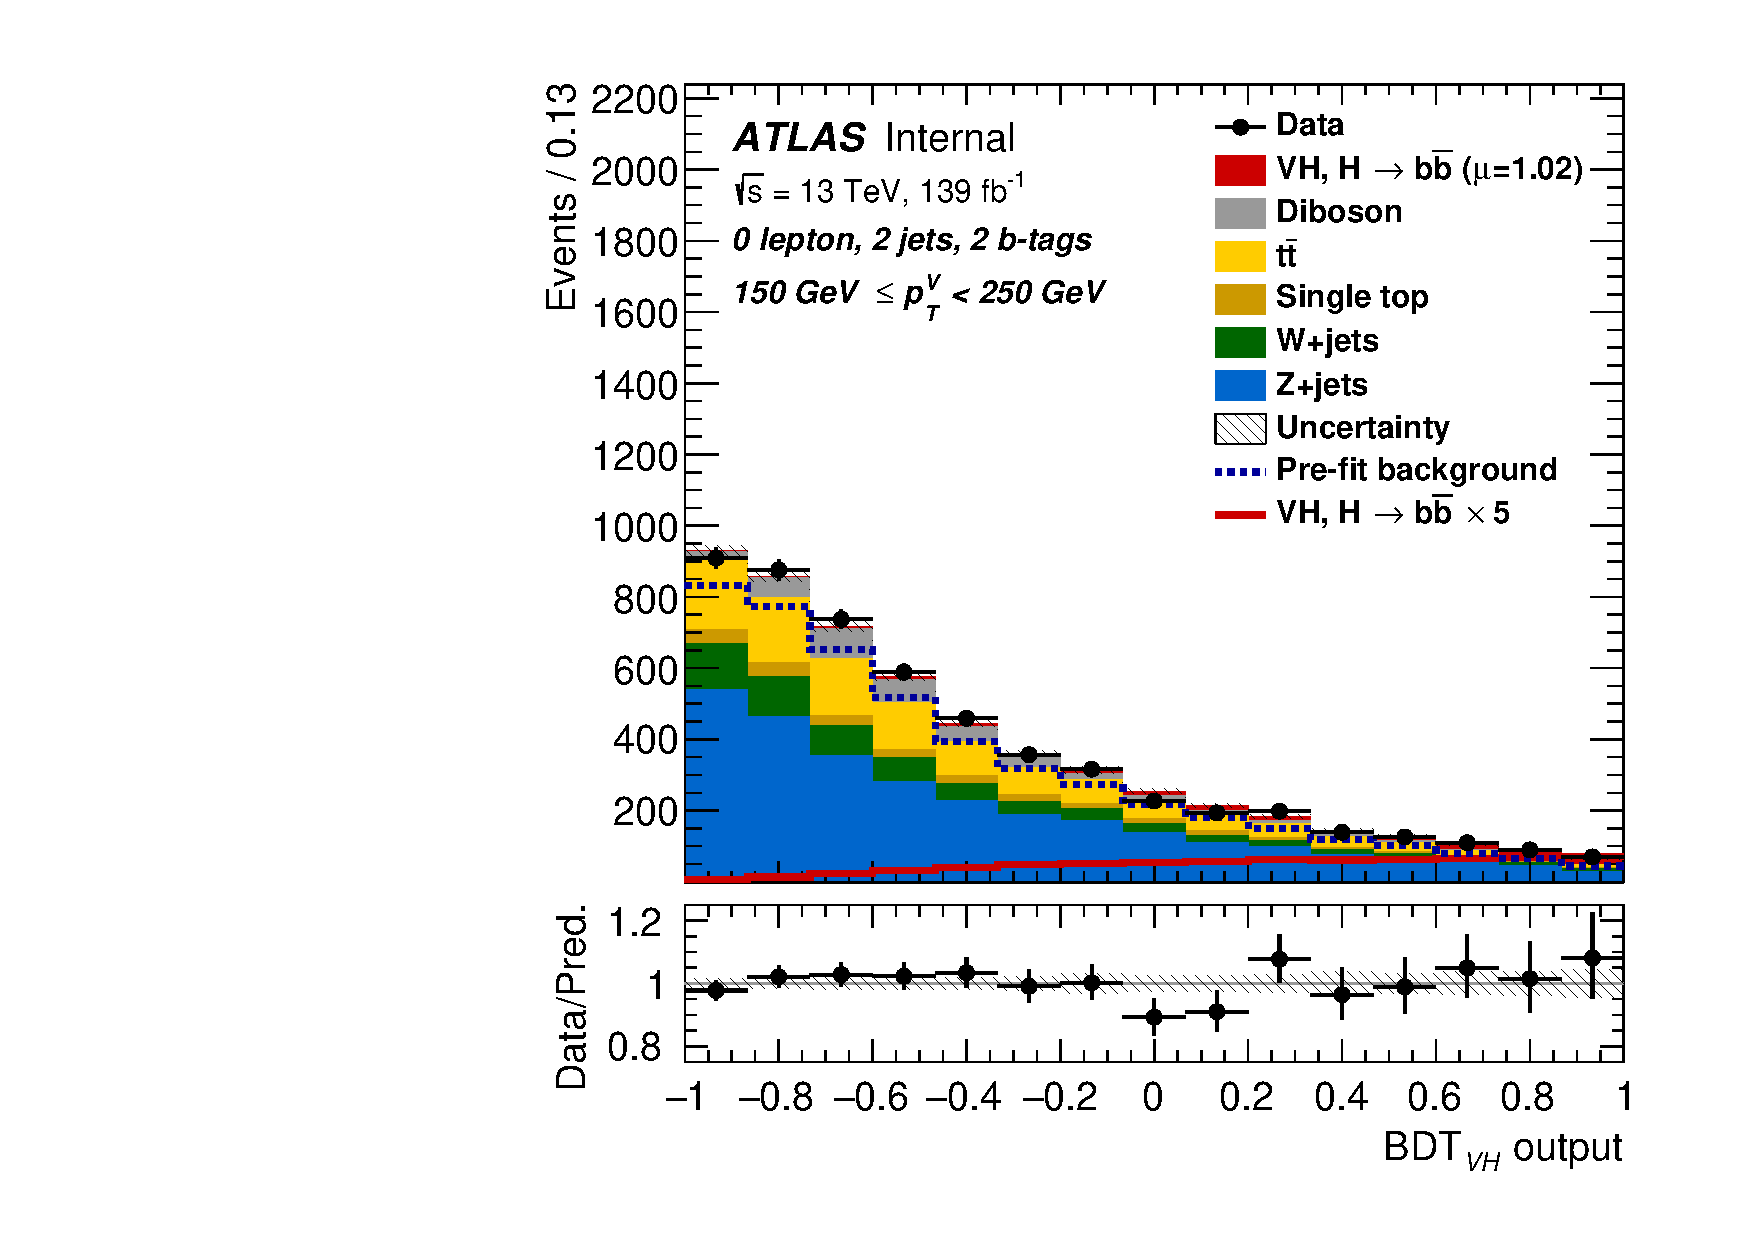
\includegraphics[width=.49\textwidth]{final_fit_mva/postfit/Region_BMax250_BMin150_Y6051_DSR_T2_L0_distmva_J2_GlobalFit_unconditionnal_mu1}%
    & 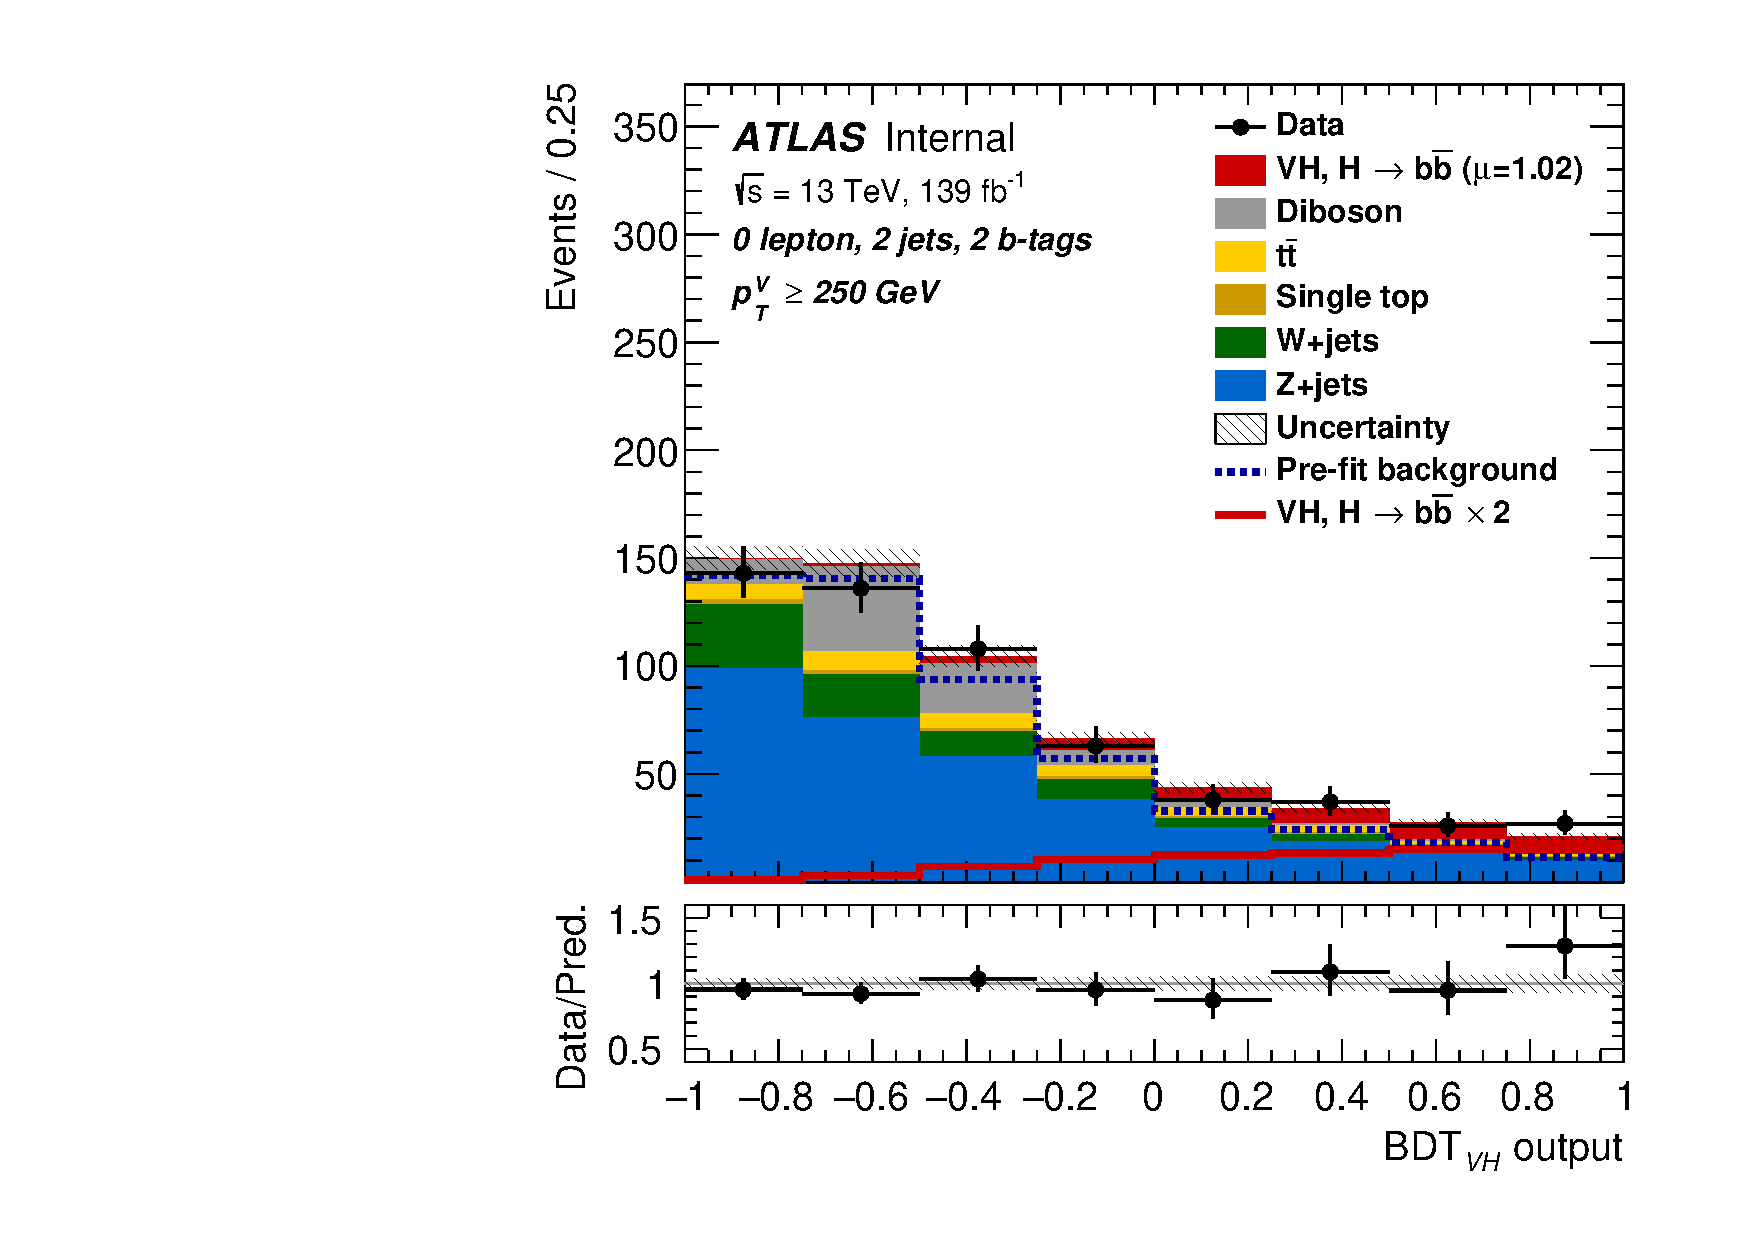
\includegraphics[width=.49\textwidth]{final_fit_mva/postfit/Region_BMin250_Y6051_DSR_T2_L0_distmva_J2_GlobalFit_unconditionnal_mu1} \\

    % bottom row
    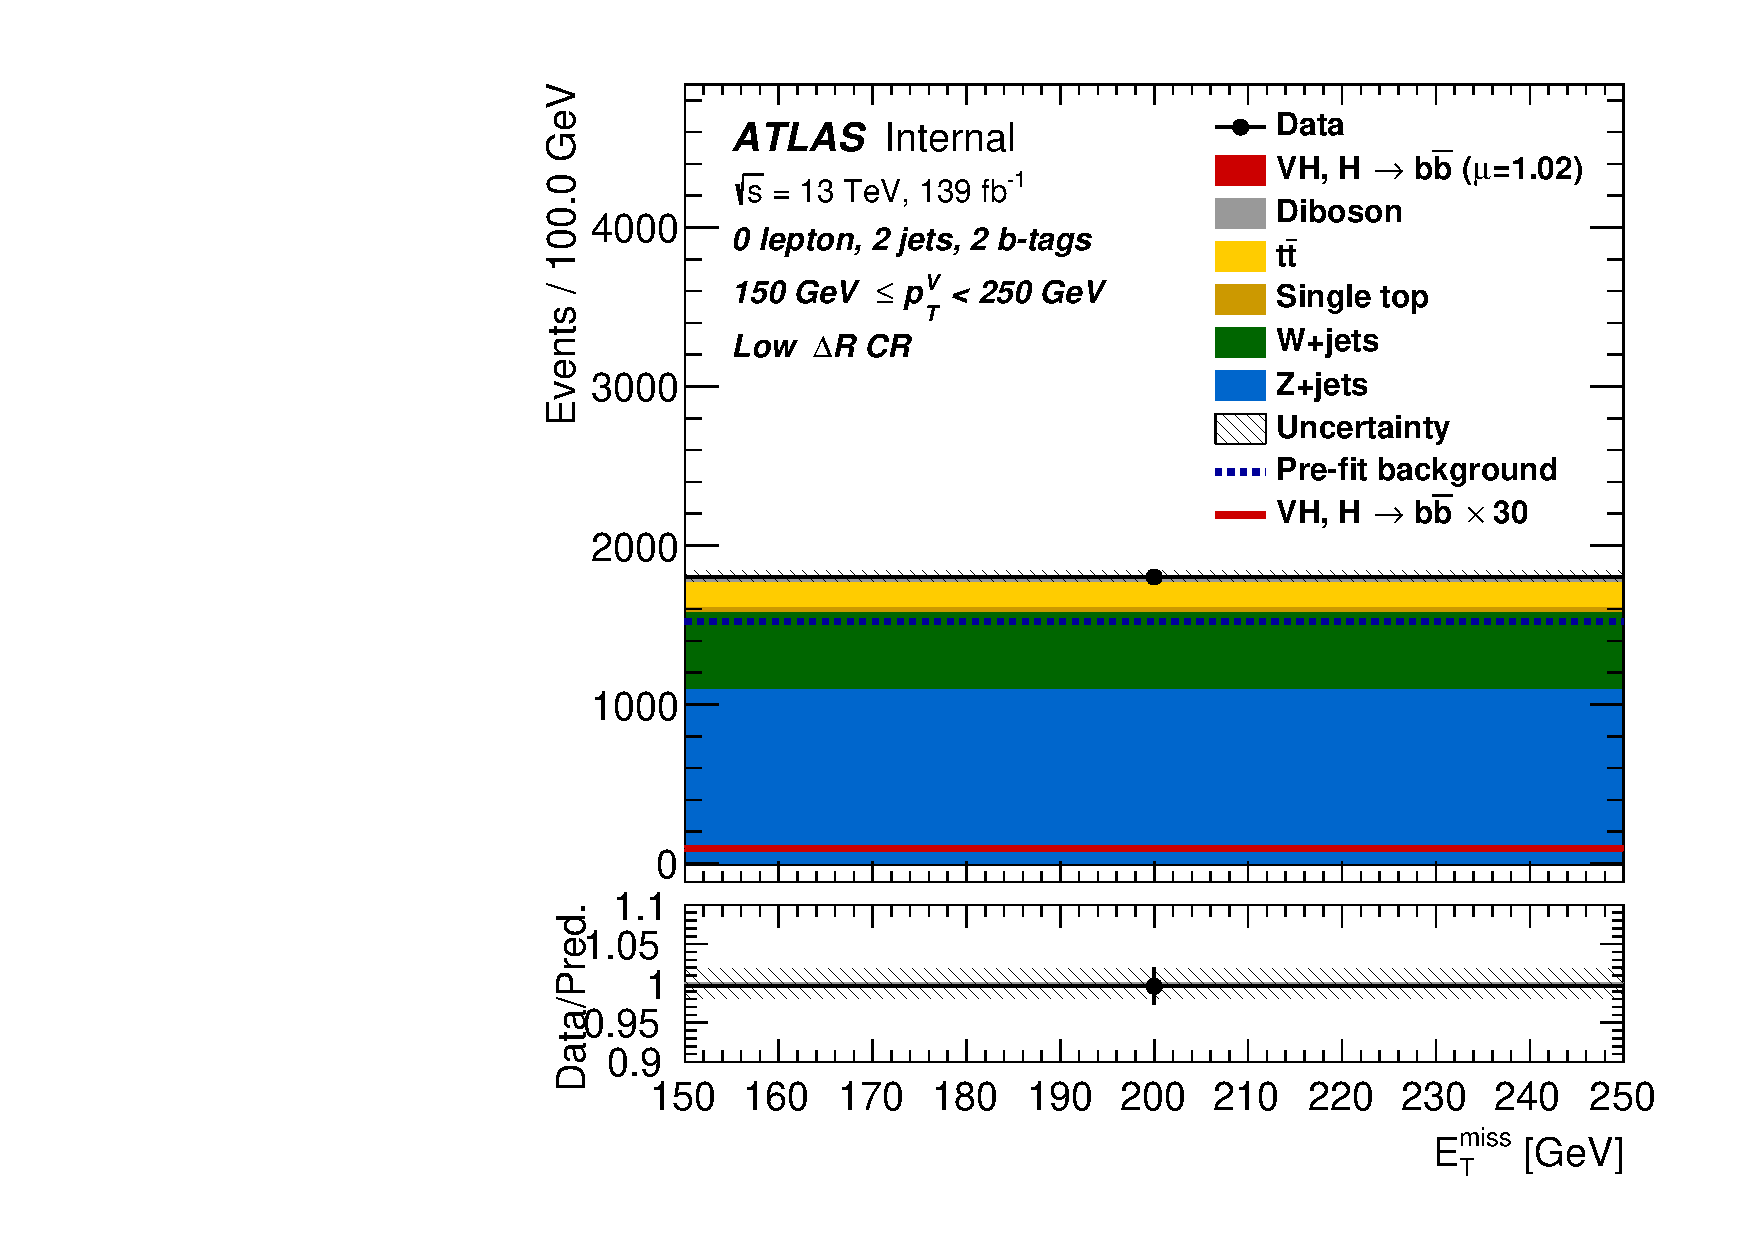
\includegraphics[width=.49\textwidth]{final_fit_mva/postfit/Region_BMax250_BMin150_Y6051_DCRLow_T2_L0_distMET_J2_GlobalFit_unconditionnal_mu1}%
    & 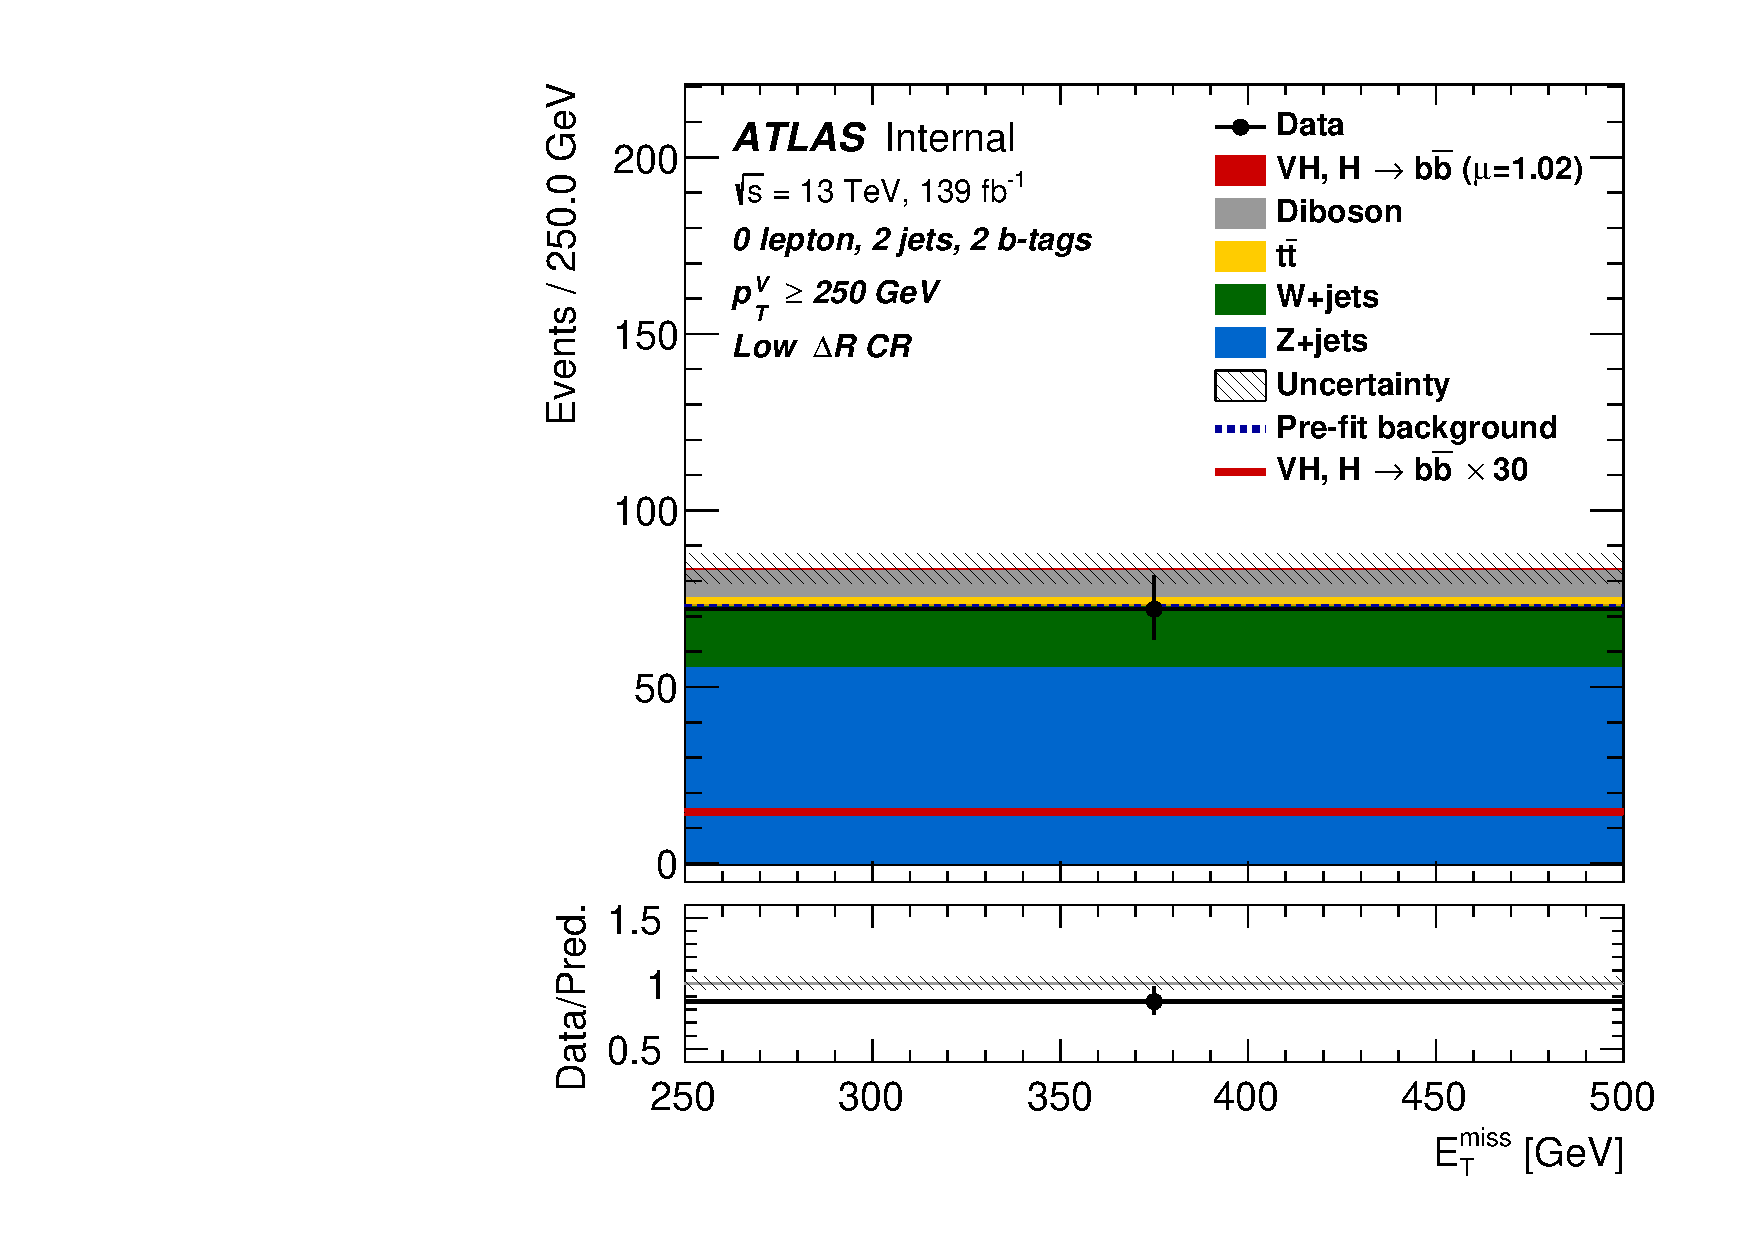
\includegraphics[width=.49\textwidth]{final_fit_mva/postfit/Region_BMin250_Y6051_DCRLow_T2_L0_distMET_J2_GlobalFit_unconditionnal_mu1} \\
  \end{tabular}
  \caption{Post-fit distributions in the 0--lepton 2--jet channel.}
  \label{fig:0lep2jet-postfit}
\end{figure}